\section{Design of \sys}
\label{s:impl}

\sys is a coverage-directed concurrency fuzzer to effectively discover
kernel concurrency bugs.
%
The key improvement of \sys lies in adopting interleaving segment
coverage and the coverage-directed interleaving search strategy
described in \autoref{s:design}.
%

As shown in \autoref{fig:workflow}, \sys consists of two stages of
fuzzing similar with recent concurrency fuzzings~\cite{razzer,
  snowboard}.
%
The first stage is a \textit{single-thread fuzzing}, which focuses on
identifying two system calls that may expose new interleaving
segments.
%
The second stage is a \textit{multi-thread fuzzing} to explore thread
interleavings and discover concurrency bugs.
%
In both stage, \sys traces timestamp-annotated memory accesses
executed by each system call for probing unobserved interleaving
segments.
%
And in the second stage, \sys adopts a mechanism to control thread
scheduling as desired.



In the following, we provide the overall design of
\sys~(\autoref{ss:fuzzer}).
%
Then, we describe the target kernel
instrumentation~(\autoref{ss:instrumentation}) to trace memory
accesses, and the execution engine~(\autoref{ss:engine}) to control
thread scheduling.
%
Lastly, we explain the implementation detail of
\sys~(\autoref{ss:impl}).




\subsection{Userspace Fuzzer}
\label{ss:fuzzer}



\begin{figure}
  \centering
  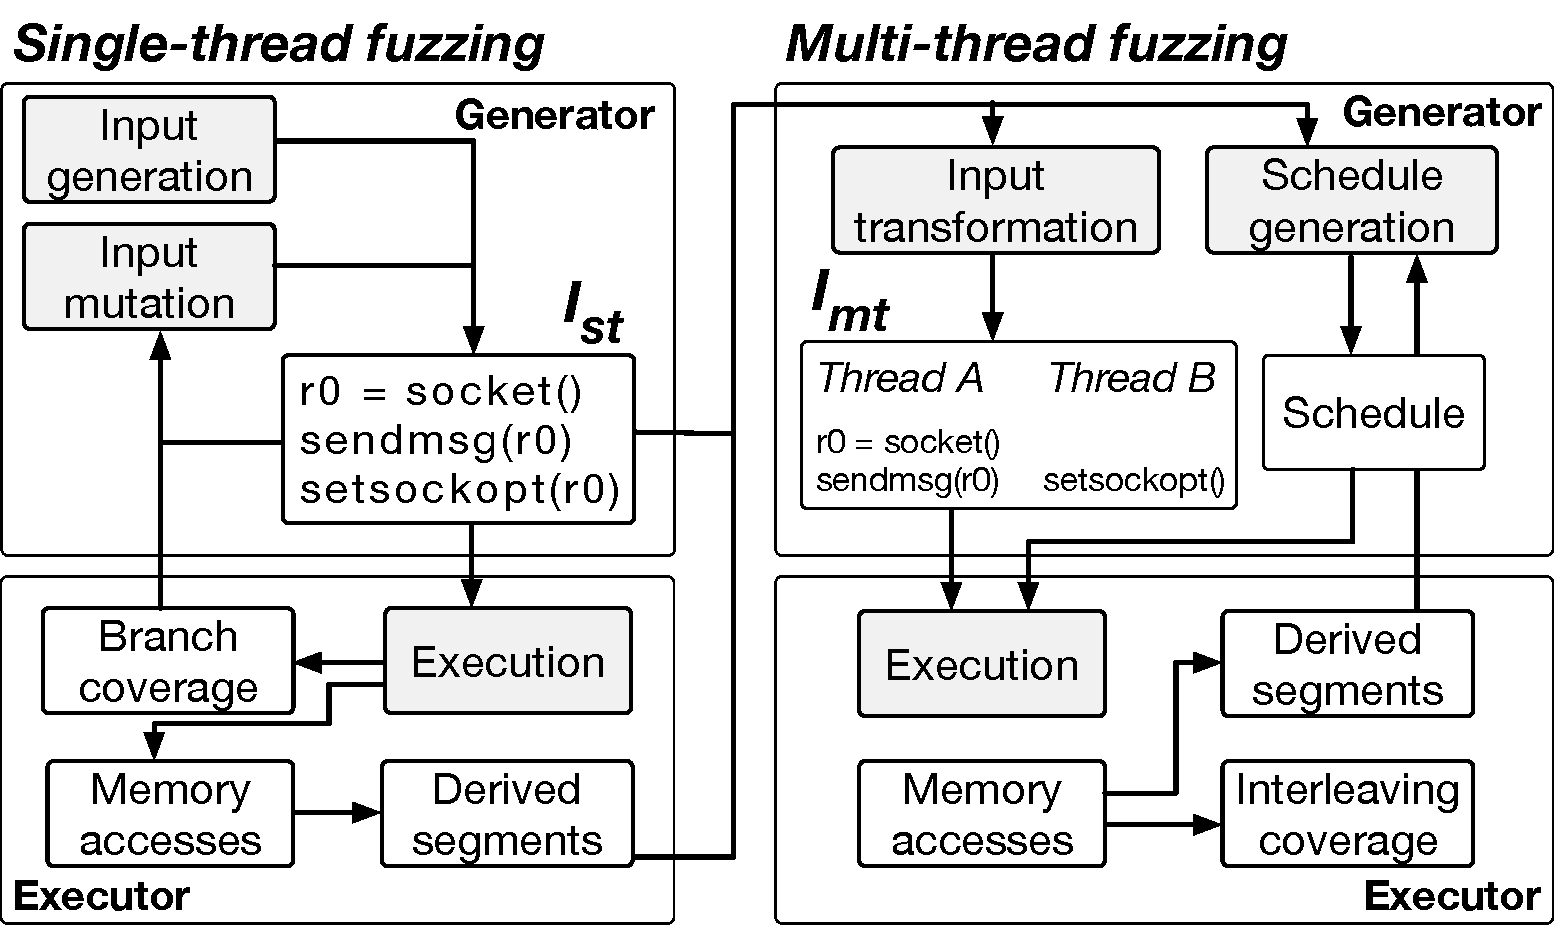
\includegraphics[width=\linewidth]{fig/architecture.pdf}
  \caption{An overview of \sys's architecture.}
  \label{fig:workflow}
\end{figure}


\sys's single-thread fuzzing~(\autoref{sss:singlethreadfuzzing}) and
multi-thread fuzzing~(\autoref{sss:multithreadfuzzing}) consist of two
components, an input generator and an input executor. We explain
details of each component in the following.


\subsubsection{Single-thread fuzzing}
\label{sss:singlethreadfuzzing}
%
In a single-thread fuzzing stage, the \textit{single-thread generator}
produces a single-thread input (referred as $I_{ST}$) in the form of a
sequence of random system calls.
%
And then, the \textit{single-thread executor} runs $I_{ST}$ to perform
two things.
%
First, it tracks code coverage of $I_{ST}$ as conventional fuzzing
does. Second, it identifies two system calls in $I_{ST}$ that
potentially exhibit new interleaving segment coverage.  If identified,
$I_{ST}$ will be passed to the next stage, the multi-thread fuzzing.


\PP{Single-thread generator}
%
Similar with a conventional fuzzing, the single-thread generator
constructs a single-threaded system call sequence $I_{ST}$ with two
strategies, generation and mutation.
%
When using the generation strategy, \sys randomly generates a system
call sequence based on well-formed system call description grammar
\texttt{Syzlang}~\cite{syzlang}.
%
\texttt{Syzlang} describes templates of available system calls
including types of arguments and the type of a return value, as well
as a range of feasible values of each argument.
%
According to \texttt{Syzlang}, \sys produces a single-thread system
call sequence by repeatedly selecting a random system call and
providing reasonable arguments of the system call.

The mutation strategy is an alternative of the generation strategy.
When using a mutation strategy, \sys picks up an already-generated
single-thread input, and modifies the single-thread input by appending
additional system calls, removing existing system calls, or changing
values of arguments of existing system calls.


\PP{Single-thread executor}
%
Given $I_{ST}$ from the single-thread generator, the single-thread
executor runs $I_{ST}$.
%
During the execution, the single-thread executor traces basic blocks
and memory accesses executed by each system call with a support from
instrumentation detailed in \autoref{ss:instrumentation}.

With traced basic blocks and memory accesses, the single-thread
executor conducts two tasks.
%
The first task is to computes branch coverage using traced basic
blocks.
%
If $I_{ST}$ exposes new branch coverage that has not been explored,
\sys keeps $I_{ST}$, and feeds it back to the single-thread generator
so that the single-thread generator further mutates $I_{ST}$ to find
more branch coverage.


Second, the single-thread executor identifies a pair of system calls
in $I_{ST}$ that potentially exposes new interleaving segment coverage
if executed concurrently.
%
More specifically, for each system call pair ($S_i$, $S_j$) in
$I_{ST}$, the single-thread executor constructs a set of explored
interleaving segment graphs $G$ (as described in
\autoref{ss:coverage}). Then, by mutating $g \in G$ (as described in
\autoref{ss:scheduler}), the single-thread executor generates a set of
unexplored segment graphs $G_{mutated}$ between ($S_i$, $S_j$).
%
If $G_{mutated}$ is not empty, the single thread executor passes
$I_{ST}$ as well as ($S_i$, $S_j$) and $G_{mutated}$ to the next
phase, the multi-thread fuzzing.




% It is worth noting that $S_i$ and $S_j$ were executed
% \textit{sequentially}.
%
% However, the single-thread executor still can
% generate interleaving segment graphs from $S_i$ and $S_j$ in a form
% similar to \autoref{fig:interleavingsegmentgraph}. \dr{TODO: rewrite}



% Instead, the single-thread executor makes use of $G$ to derive
% a set of \textit{unobserved} interleaivng segment graphs
% $G^{derived}$.
% %
% To this end, for each interleaving segment graph $g \in G$,
% the single-thread executor derives new interleaving segment graphs
% (refer to \autoref{fig:interleavingmutation}), and puts ones that
% unobserved before in $G^{derived}$.
% %
% Lastly, if $G^{derived}$ is not empty, the single thread executor
% passes $I_{ST}$ as well as ($S_i$, $S_j$) and $G^{derived}$ to the
% next phase, the multi-thread fuzzing.


% The single-thread executor does not record $G$ in the
% interleaving segment coverage because $S_i$ and $S_j$ were executed
% sequentially.


\subsubsection{Multi-thread fuzzing}
\label{sss:multithreadfuzzing}
%
After $I_{ST}$ is passed with ($S_i$, $S_j$) and
$G^{derived}_{(i,j)}$, the \textit{multi-thread generator} transforms
$I_{ST}$ to a multi-thread input $I_{MT}$.
%
In addition, the multi-thread generator produces \textit{schedules}
where each schedule describes how to enforce thread interleaving
during runtime.
%
The \textit{multi-thread executor} then repeatedly tests each schedule
of $I_{MT}$ one at a time with a support of the execution
engine~(\autoref{ss:engine}).


\PP{Schedule}
%
A schedule is a specification of how to control thread scheduling.
%
It contains a starting system call and per-system call sequences of
scheduling points that each scheduling point is described as a
two-tuple (instruction address, scheduling order).

\begin{figure}[t]
  \centering
  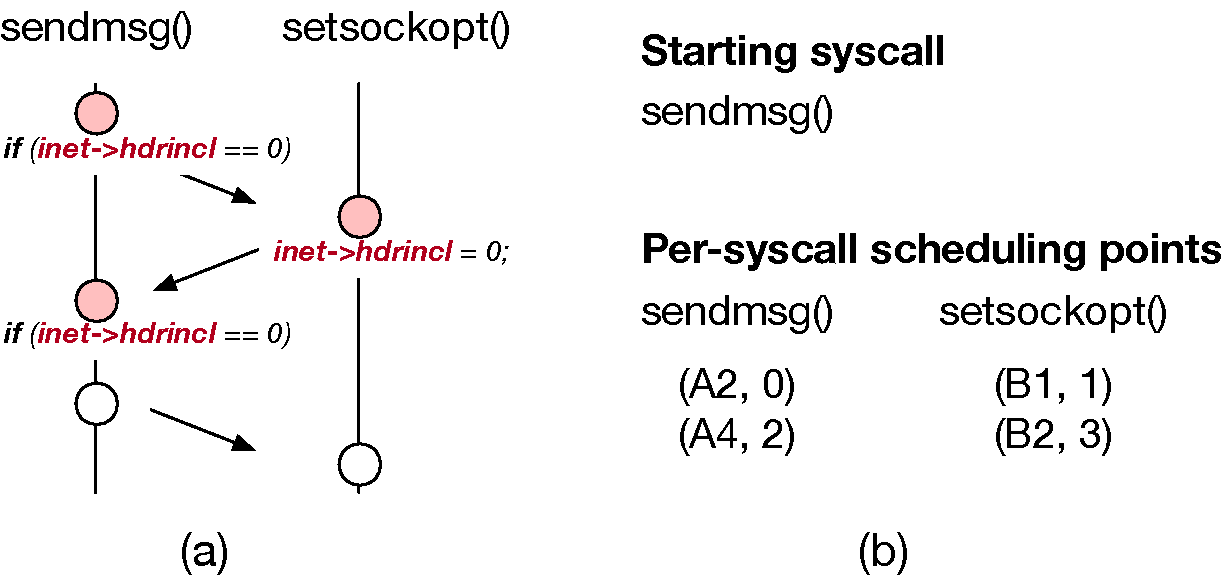
\includegraphics[width=0.75\linewidth]{fig/schedule.pdf}
  \caption{(a) Thread interleaving, and (b) schedule to run thread
    interleaving of (a).}
  \label{fig:schedule}
\end{figure}

\autoref{fig:schedule} illustrates an example of a schedule. In order
to run a thread interleaving in \autoref{fig:schedule}-(a), the
execution should start with \texttt{sendmsg()}. So the schedule states
that a starting syscall is \texttt{sendmsg()}.
%
Then, in \autoref{fig:schedule}-(a), three preemptions (excluding the
end of system calls) are required at \texttt{A2}, \texttt{B1}, and
\texttt{A4}. Each schedule point denotes an instruction on which a
preemptions occurs, annotated with the order of preemption.


%During fuzzing, the userspace fuzzer keeps generating different
%schedules, and requests the execution engine through hypercall
%interfaces to control thread scheduling according to a schedule.




\PP{Multi-thread generator}
%
% In order to use interleaving graph as interleaving coverage, we need a
% method to store them, and compare them to a new interleaving graph.
% %
% We choose to use a hash value of
%
% the FNV-1~\cite{fnv, fnv-go}, non-cryptographic hash function,
%
%
% A schedule is an outcome of the interleaving mutation.
% A schedule contains an initial thread, and a set of scheduling points
% indicating an instruction on which preemption occurs.
%
The multi-thread generator has two roles, 1) transforming $I_{ST}$
into a multi-thread input $I_{MT}$ and 2) generating various
schedules.





% \begin{figure}[t]
%   \scriptsize
%   \centering
%   \begin{Verbatim}[commandchars=\\\{\},codes={\catcode`\$=3\catcode`\^=7\catcode`\_=8\relax}]
\PY{k}{def} \PY{n+nf}{Convert\PYZus{}Pst\PYZus{}to\PYZus{}Pmt}\PY{p}{(}\PY{n}{Pst}\PY{p}{,} \PY{n}{i}\PY{p}{,} \PY{n}{j}\PY{p}{,} \PY{n}{RP\PYZus{}i}\PY{p}{,} \PY{n}{RP\PYZus{}j}\PY{p}{)}\PY{p}{:}
    \PY{c+c1}{\PYZsh{} @Pst: A singled threaded program (annotated)}
    \PY{c+c1}{\PYZsh{} @i, @j: an index of racing syscalls within Pst}
    \PY{c+c1}{\PYZsh{} @RP\PYZus{}i, @RP\PYZus{}j: an address of a corresponding racepair}
    \PY{c+c1}{\PYZsh{} instruction (to syscalls[i] and syscalls[j], respectively)}

    \PY{c+c1}{\PYZsh{} Get pinned threads, thr0 and thr1}
    \PY{n}{thr0} \PY{o}{=} \PY{n}{get\PYZus{}pinned\PYZus{}thread}\PY{p}{(}\PY{n}{vCPU0}\PY{p}{)}
    \PY{n}{thr1} \PY{o}{=} \PY{n}{get\PYZus{}pinned\PYZus{}thread}\PY{p}{(}\PY{n}{vCPU1}\PY{p}{)}

    \PY{c+c1}{\PYZsh{} Assign syscalls to thr0 and thr1}
    \PY{n}{syscalls} \PY{o}{=} \PY{n}{get\PYZus{}syscalls}\PY{p}{(}\PY{n}{Pst}\PY{p}{)}
    \PY{n}{thr0}\PY{o}{.}\PY{n}{add\PYZus{}syscalls}\PY{p}{(}\PY{n}{syscalls}\PY{p}{[}\PY{p}{:}\PY{n}{i}\PY{p}{]}\PY{p}{)}
    \PY{n}{thr1}\PY{o}{.}\PY{n}{add\PYZus{}syscalls}\PY{p}{(}\PY{n}{syscalls}\PY{p}{[}\PY{n}{i}\PY{o}{+}\PY{l+m+mi}{1}\PY{p}{:}\PY{n}{j}\PY{p}{]}\PY{p}{)}

    \PY{c+c1}{\PYZsh{} Determine the execution order}
    \PY{n}{r} \PY{o}{=} \PY{n}{random}\PY{p}{(}\PY{p}{[}\PY{n}{vCPU0}\PY{p}{,} \PY{n}{vCPU1}\PY{p}{]}\PY{p}{)}
    \PY{n}{thr0}\PY{o}{.}\PY{n}{add\PYZus{}hypercall}\PY{p}{(}\PY{n}{hcall\PYZus{}order}\PY{p}{(}\PY{n}{r}\PY{p}{)}\PY{p}{)}

    \PY{c+c1}{\PYZsh{} Trigger and check races}
    \PY{n}{thr0}\PY{o}{.}\PY{n}{add\PYZus{}hypercall}\PY{p}{(}\PY{n}{hcall\PYZus{}set\PYZus{}bp}\PY{p}{(}\PY{n}{vCPU0}\PY{p}{,} \PY{n}{RP\PYZus{}i}\PY{p}{)}\PY{p}{)}
    \PY{n}{thr0}\PY{o}{.}\PY{n}{add\PYZus{}syscalls}\PY{p}{(}\PY{n}{syscalls}\PY{p}{[}\PY{n}{i}\PY{p}{]}\PY{p}{)}
    \PY{n}{thr0}\PY{o}{.}\PY{n}{add\PYZus{}hypercall}\PY{p}{(}\PY{n}{hcall\PYZus{}check}\PY{o}{\PYZhy{}}\PY{n}{race}\PY{p}{(}\PY{p}{)}\PY{p}{)}

    \PY{n}{thr1}\PY{o}{.}\PY{n}{add\PYZus{}hypercall}\PY{p}{(}\PY{n}{hcall\PYZus{}set\PYZus{}bp}\PY{p}{(}\PY{n}{vCPU1}\PY{p}{,} \PY{n}{RP\PYZus{}j}\PY{p}{)}\PY{p}{)}
    \PY{n}{thr1}\PY{o}{.}\PY{n}{add\PYZus{}syscalls}\PY{p}{(}\PY{n}{syscalls}\PY{p}{[}\PY{n}{j}\PY{p}{]}\PY{p}{)}
    \PY{n}{thr1}\PY{o}{.}\PY{n}{add\PYZus{}hypercall}\PY{p}{(}\PY{n}{hcall\PYZus{}check\PYZus{}race}\PY{p}{(}\PY{p}{)}\PY{p}{)}

    \PY{c+c1}{\PYZsh{} Post\PYZhy{}race behaviors}
    \PY{n}{thr0}\PY{o}{.}\PY{n}{add\PYZus{}syscalls}\PY{p}{(}\PY{n}{gen\PYZus{}random\PYZus{}syscalls}\PY{p}{(}\PY{p}{)}\PY{p}{)}
    \PY{n}{thr1}\PY{o}{.}\PY{n}{add\PYZus{}syscalls}\PY{p}{(}\PY{n}{gen\PYZus{}random\PYZus{}syscalls}\PY{p}{(}\PY{p}{)}\PY{p}{)}

    \PY{n}{Pmt} \PY{o}{=} \PY{n}{Construct\PYZus{}Pmt}\PY{p}{(}\PY{n}{thr0}\PY{p}{,} \PY{n}{thr1}\PY{p}{)}
    \PY{k}{return} \PY{n}{Pmt}
\end{Verbatim}

%   \caption{\sys's multi-thread generator algorithm. \dr{Seems too
%       much}}
%   \label{f:mt-conversion}
% \end{figure}
%
Given $I_{ST}$ and ($S_i$, $S_j$), the multi-thread generator produces
$I_{MT}$ which preserves all system calls in $I_{ST}$, but executes
$S_i$ and $S_j$ concurrently.
%
Assuming, $0 < i < j < n$, where n is the total number of syscalls in
$I_{ST}$, the input transformation is simply done by dividing
$I_{ST}$ into two parts.

%
Then, the multi-thread generator assigns XXX to thread0, and YYY to
thread1.




On the other hand, the multi-thread generator repeatedly produces
various schedules.
%
To generating schedules, the multi-thread generator takes
$G^{derived}_{(i,j)}$ as input.
%
Then, for each repetition, the multi-thread generator selects a subset
of $G^{derived}_{(i,j)}$, $G^{*}_{(i,j)}$, that are XXX.






\PP{Multi-thread executor}
%
The multi-thread executor runs $I_{MT}$ while enforcing a schedule
generated by the multi-thread generator.
%
To this end, the multi-thread executor spawns multiple threads and
assigns system calls to the threads.
%
Each thread then runs an assigned system call concurrently, while
the execution engine~(\autoref{ss:engine}) enforces a given schedule.


During the execution of $I_{MT}$, \sys checks that the running thread
interleaving causes a harmful behavior such as memory corruption or
deadlock.
%
For this, \sys relies on various devloper tools such as assertions in
the kernel, lockdep~\cite{lockdep}, kernel watchdog~\cite{watchdog}, and
sanitizers~\cite{kasan, ubsan, asan}.
%
If these developer tools detect that an abnormal behavior occurs in
the kernel, \sys writes a report of the abnormal behavior as well as
$I_{MT}$ and the executed thread interleaving.







If $I_{MT}$ is executed without causing an abnormal behavior, the
multi-thread executor collects memory accesses that racing system
calls executed.
%
With these memory accesses, the multi-thread executor probes for
interleaving segment coverage as described in
\autoref{ss:coverage}. In addition, it derives more unobserved
interleaving segment graphs as the single-thread executor does, and
feeds unobserved interleaving segment graphs to the multi-thread
generator to further explore thread interleavings.







\subsection{Target Kernel Instrumentation}
\label{ss:instrumentation}

\sys requires to trace basic blocks (for tracking code coverage) and
timestamp-annotated memory accesses (for tracking interleaving
coverage) executed by each system call.
%
For this, \sys incorporates a compiler pass that inserts callback
function calls 1) at the beginning of each basic block, and 2) before
each instruction that accesses globally-visible memory objects.
%
% These callback functions record executed basic blocks and memory
% accesses into per-thread memory regions shared between the user space
% and the kernel space. Thus after a thread executes a system call, the
% thread can identify basic blocks and memory accesses that it executed.



\begin{figure}
  \centering
  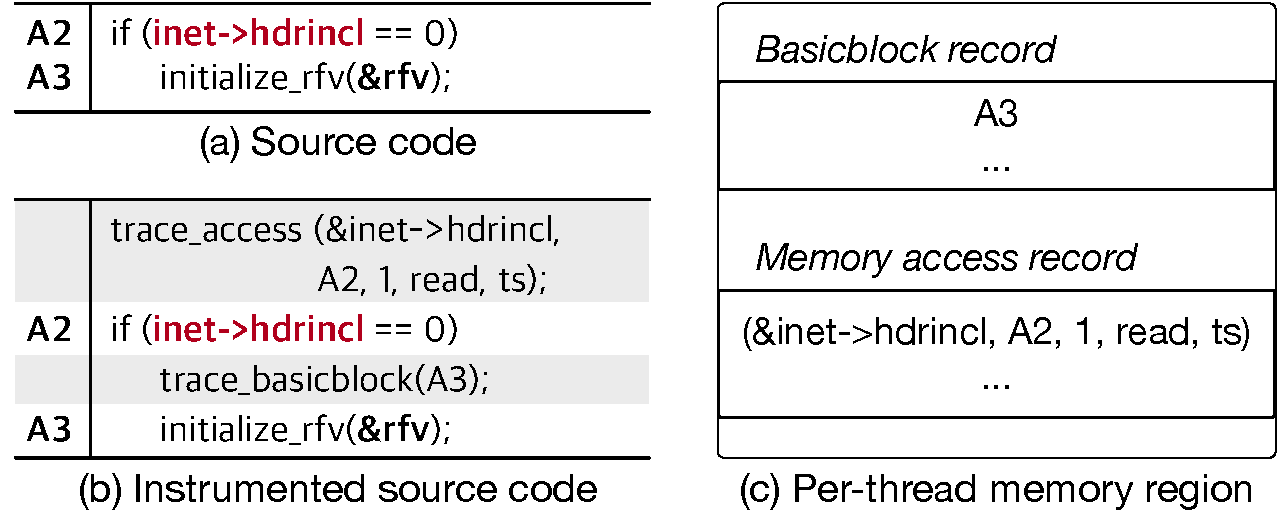
\includegraphics[width=0.9\linewidth]{fig/instrumentation.pdf}
  \caption{(a) Part of \texttt{raw_sendmsg()} in
    \autoref{fig:cve-2017-17712}, (b) instrumented source code of (a)
    (gray on the background), and (c) memory accesses and basic blocks
    recorded during runtime.}
  \label{fig:instrumentation}
\end{figure}

\autoref{fig:instrumentation} shows how the \sys's compiler pass
inserts callbacks, and how each callback records memory accesses and
basic blocks.
%
When compiling a source code in (a), the compiler pass two inserts
function calls; \texttt{trace_basicblock()} before \texttt{A3} which
is the first instruction of the basic block, and
\texttt{trace_access()} before \texttt{A2} which is an instruction
that accesses \texttt{inet->hdrincl}.


During runtime, \texttt{trace_basicblock()} takes the starting address
of basic block as input (\ie, \texttt{A3}), and records it into
\texttt{Basicblock record}.
%
On the other hand, \texttt{trace_access()} takes five parameters, the
address of the accessed memory object (\ie, \texttt{\&inet->hdrincl}),
the instruction address accessing the memory object (\ie,
\texttt{A2}), the size of the memory access (\ie, \texttt{1}), the
type of the memory access (\ie, \texttt{read}), and the timestamp of
when the memory access occurrs (\ie, \texttt{ts}).
%
\texttt{trace_access()} then records these five parameters into
\texttt{Memory access record}.






% It is worth noting that \texttt{Basicblock record} and \texttt{Memory
%   access record} are per-thread memory regions, shared between the
% user space and the kernel space. Thus, after a userspace thread
% executes a system call, the thread can identify basic blocks and
% memory accesses that it executed.







% Unlike data race detectors such as KCSAN~\cite{kcsan}, the \sys's
% scheduling mechanism needs to recognize both plane memory accesses and
% annotated memory accesses such as atomic operations.
% %
% We deal with these two types of accesses differently since annotated
% accesses usually are implemented in assembly code, which is hard for a
% LLVM pass to understand.
% %
% In order to instrument plane accesses, we implement a LLVM pass that
% insert callback function calls after memory accesses on LLVM IR.
% %
% Our pass runs after most of binary transfomration is done, so it
% \XXX{...}.
% %
% For annotated instructions, we rely on the functionality of
% KASAN~\cite{kasan} to instrument atomic operations.
% %
% KASAN provides wrapper functions of annotation APIs to call callback
% functions before annotated memory operations, and we instruct the
% wrapper functions to call our callbacks as well.
% %
% Our callbcak functions write memory access operations along with
% various information into a region mmap-ed shared region shared by a
% userspace program (\ie, fuzzer) and a kernel. The information about
% memory operations includes the instruction address, the start address
% of a memory location, and the size of memory access.
% %
% Accordingly, a fuzzer is able to identify what memory access
% operations took place during the execution.

% \sys also requires an additional module called a trampoline that is
% used to suspend and resume a running thread. Details about the
% trampoline are described in \autoref{ss:engine}.


\subsection{Execution Engine}
\label{ss:engine}

\sys introduces an execution engine in order to grant an ability to
the userspace fuzzer that it can control thread scheduling.
%
The execution engine is implemented in the hypervisor layer to be
non-intrusive to the kernel execution.




In order to monitor the kernel execution, \sys leverages the hardware
breakpoint feature~\cite{hwbp} shipped in modern Intel CPU chipsets.
%
The execution engine installs breakpoints on instructions on which
scheduling points refer, and recognizes that a thread of the userspace
fuzzer reaches a scheduling point when a breakpoint is hit.
%


\dr{I'm rewriting this part to shrink}

\PP{Enforcing a schedule}
%
In order for the userspace fuzzer to ask the execution engine to
enforce a schedule, the userspace fuzzer sends a schedule to run
thorugh hypercall interfaces.
%
After that, the threads notify the execution engine that they are
ready to execute system calls, and start executing system calls,
%
During the execution, the execution engine keeps only one thread to
run, and deliberately suspends and resumes the execution of system
calls according to the given schedule.

%
\begin{figure}[t]
  \centering
  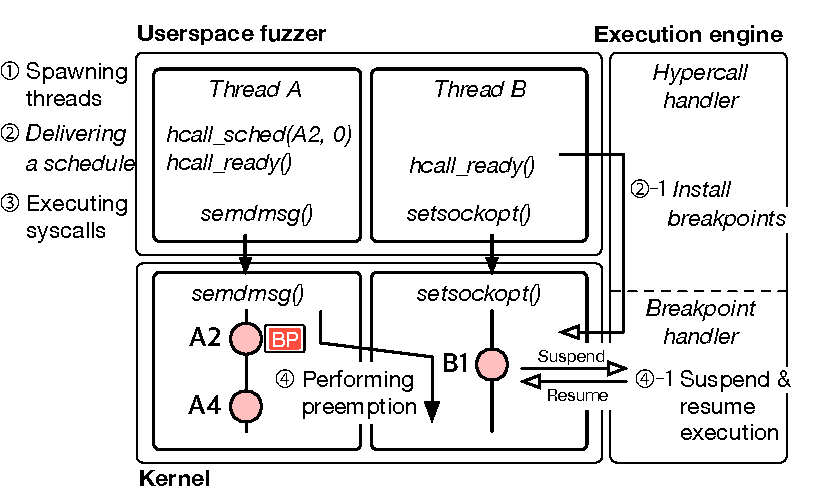
\includegraphics[width=0.9\linewidth]{fig/workflow-hypervisor.pdf}
  \caption{The workflow of the execution engine. \red{IMPORTANT: this
      is copied from AITIA. Need to redraw}}
  \label{fig:workflow-hypervisor}
\end{figure}
%
\autoref{fig:workflow-hypervisor} shows a workflow of the execution
engine.
%
At the beginning, the userspace fuzzer spawns threads, where each
thread is assigned a system call annotated with scheduling points
(\C{1} in \autoref{fig:workflow-hypervisor}).
%
Then, each thread invokes hypercalls to deliver scheduling points to
the execution engine (\C{2}). In \sys, three types of hypercalls are
used; \texttt{hcall_XXX()} to inform the starting system call,
\texttt{hcall_sched()} to deliever a single scheduling point, and
\texttt{hcall_ready()} to notify that a calling thread is ready.
%
Also, \texttt{hcall_ready()} sleeps until all threads all threads are
ready. When all threads invoke \texttt{hcall_ready()}, the execution
engine wakes them up, and the threads start executing system calls
(\C{3}).

\dr{installing BPs}


During the execution of system calls, only one thread is allowed to
run. In \autoref{fig:workflow-hypervisor}, thread~A (\ie,
\texttt{sendmsg()}) runs first because it is a starting system
call (\ie, it called \texttt{hcall_XXX()}).
%
Because a breakpoint is installed on \texttt{A2}, the execution engine
is noticed that thread~A reaches \texttt{A2}.
%
Then, the execution engine suspends thread~A, and switches to exeucte
thread~B.
%
To suspend thread~A, the execution enigne stores context information
(\eg, register values) in the hypervisor's memory, and changes the
program counter of thread~A to an infinite loop called a trampoline.
%
In the trampoline, thread~A keeps calling \texttt{cond_resched()} to
yield a CPU without proceeding with the system call execution, thus
thred~A is confined in the trampoline.
%

\PP{Performing preemption}



While thread~A is confined in the trampoline, thread~B runs its system
call \texttt{setsockopt()}.
%
But another breakpoint is installed on \texttt{B1}, when thread~B
reaches a scheduling point (\texttt{B1}), the execution engine again
suspends thread~B and switches to execute thread~A.
%
Suspending thread~B is performed in the same way described above.
%
To resume thread~A , the execution engine restores registers with the
values of registers including a program counter saved when thread~A
was suspended. Then thread~A can continue its execution.


The execution engine keeps suspending and resuming system calls until
one of the two threads finishes its execution. In this example,
thread~A finishes its execution first, and notifies the end of
execution to the execution engine through \texttt{hcall_done()}.
%
Upon receiving \texttt{hcall_done()}, the execution engine resumes the
suspended thread (\ie, thread~B) and lets it finish its execution.




\PP{Restriction of hardware breakpoint}
%
While a hardware breakpoint feature is well-fitting for our pupose, it
has a restriction on the number of breakpoints that can be installed
at the same time.
%
In Intel CPU chipsets, at most four hardware breakpoints can be
installed simultaneously, and the number of scheduling points can be
larger than four.
%
\sys overcomes this restriction by leveraging the fact that
scheduling points are ordered. In other words, the execution engine
installs breakpoints on a first few (\eg, four) scheduling points,
and when a installed breakpoint is hit, the execution engine moves a
breakpoint onto the next scheduling point.
%
Also we expect that this restriction can be further mitigated by using
architectures with more hardware breakpoints (\eg, ARM v7 equipped six
hardware breakpoints), or using a software breakpoint feature that
does not have a restriction on the number of breakpoints.



%\dr{not important. i'm thinking remove this}
%
%In performing preemption, we choose to suspend and resume a guest
%thread instead of a whole virtual CPU on which the guest thread runs.
%
%While suspending and resuming a whole virtual CPU is adopted by
%previous approaches~\cite{ski, snowboard, razzer} it is not suitable
%for our purpose because \textit{if suspending a virtual CPU, it may
%  suspend another virtual CPU}. Details are explained in the appendix
%section~(\autoref{s:appendix:preemption}).




\PP{Handling missing scheduling points}
%
It is worth noting that instructions on which scheduling points
install may not be executed if the control flow changes due to kernel internal states.
%
\dr{}In such case, we keep the order of scheduling points.
%
For example, when executing a schedule of \autoref{fig:schedule}, it is possible that thread~A may not execute \texttt{A2}, and hit a breakpoint on \texttt{A6}.
%
Then, we ignore all scheduling points before \texttt{A6} (\ie, \texttt{A2} and \texttt{B1}), and keep
enforcing a schedule after \texttt{A6} (\ie, \texttt{B2}).



\PP{Virtual Machine Instrospection}
%
While controlling thread scheduling of system calls, the execution
engine introspects the target kernel for two reasons.
%
First, because a hardware breakpoint does not distinguish which thread
hits the breakpoint, the execution engine needs to determine whether
the breakpoint is hit by a thread of the userspace fuzzer, or by an
irrelevant thread.
%
If a breakpoint is hit by a thread of the userspace fuzzer, the
execution engine suspends the thread and resumes the
previously-suspended thread as specified in a schedule.
%
Otherwise, the execution engine ignores the breakpoint hit, and keeps
running the kernel.


Second, when a running thread tries to acquire a lock, the execution
engine inspects whether the lock is held by a suspended thread to
prevent unexpected block (\ie, both threads cannot make a progress).
%
If it is the case, the execution engine performs preemption so that
the lock-holder thread (\ie, the suspended thread) resumes the
execution, and the lock-waiting thread gets suspended.


While the virtual machine introspection is crucial to properly control
thread scheduling, we leave details of how we implement the virtual
machine introspection in the appendix
section~(\autoref{s:appendix:vmi}).




\subsection{Implementation}
\label{ss:impl}

We implement \sys in various software layers as follows:
%
The target kernel instrumentation~(\autoref{ss:instrumentation}) is
implemented in two parts, a compiler pass and callback functions. The
compiler pass is implemented on the LLVM compiler suite
12.0.1~\cite{llvm} with 323~\footnote{We use scc~\cite{scc} and
  sloccount~\cite{sloccount} to measure LoC of GO and C, C++
  respectively.} LoC in C++, and, the callback functions are
implemented in the Linux kernel source tree with 265 LoC in C.
%
The execution engine~(\autoref{ss:engine}) is implemented on QEMU
6.0.0 with 1662 LoC in C, and leverages KVM (Kernel-based Virtual
Machine) to take advantage of hardware acceleration.
%
% In addition, the trampoline is enclosed into the target kernel source
% tree as a loadable module.
%
Lastly, the \sys's userspace fuzzer~(\autoref{ss:fuzzer}) is
implemented based on \texttt{Syzkaller}~\cite{syzkaller}, a kernel
fuzzer developed by Google, with 3334 LoC in GoLang and 341 LoC in C++.



% To summarize, the target kernel
% instrumentation~(\autoref{ss:instrumentation}) is implemented with 323
% LoC in C++ (for the compiler pass) and 265 LoC in C (for callback
% functions).
% %
% The execution engine~(\autoref{ss:engine}) is implemented with 1662
% LoC in C. And the userspace fuzzer~(\autoref{ss:fuzzer}) is
% implemented with 3334 LoC in GoLang and 341 LoC in C++.

% the compiler pass is implmented in 323 lines of C++
% the callback functions are implmeneted in 265 lines of C
% the execution engine is implemented in 1662 lines of C
% the trampoline is 66 in C
% c2fuzz:
% go 3334
% C++ 341







%%% Local Variables:
%%% mode: latex
%%% TeX-master: "p"
%%% End:
